\subsection{Taxonomy and representation of generalized ellipsoids}\label{sec:taxonomy}
\secref{sec:geometric} defined a \emph{proper} (origin-centered) ellipsoid in  $\Real{p}$ by
$\mathcal{E} := \{ \vec{x}: \vec{x}\trans \mat{C} \vec{x} \le 1 \}$ that is bounded with non-empty interior (call these ``fat'' ellipsoids).
For more general purposes, particularly for statistical applications,
it is useful to give ellipsoids a wider definition.
To provide a complete taxonomy, this wider definition should also include ellipsoids that may be unbounded in some directions in $\Real{p}$
(an infinite cylinder of ellipsoidal cross-section) and
degenerate (singular) ellipsoids that are ``flat'' in  $\Real{p}$ with empty interior, such as when a 3D ellipsoid has no extent in
one dimension (collapsing to an ellipse), or in two dimensions (collapsing to a line).  These ideas are made precise below
with a definition of the \emph{signature}, $\mathcal{G}(\mat{C})$, of a generalized ellipsoid.

The motivation for this more general representation is to allow a notation for a class of generalized ellipsoids to be
algebraicly closed under operations (a) image and preimage under a linear transformation, and (b) inversion.
The goal is to be able to think about, visualize, and \emph{compute} a linear transformation of an ellipsoid with central matrix
$\mat{C}$ or its inverse transformation via an analog of $\mat{C}^{-1}$, which applies equally to unbounded
and/or degenerate ellipsoids. 
Algebraically, the vector space of $\mat{C}$ is the \emph{dual} of that of $\mat{C}^{-1}$ ($\mathcal{D}$ Ch 6) and vice-versa.
Geometrical applications can show how points, lines, and hyperplanes 
in  $\Real{p}$ are all special cases of ellipsoids.
Statistical applications concern the relationship between a predictor data ellipsoid and the
corresponding $\vec{\beta}$ confidence ellipsoid (\secref{sec:betaspace}): The $\vec{\beta}$ ellipsoid will be unbounded (some linear combinations
will have infinite confidence intervals) \emph{iff} the corresponding data ellipsoid is flat, as when $p>n$ or some predictors are collinear.

Defining ellipsoids with $\{ \vec{x}: \vec{x}\trans \mat{C} \vec{x} \le 1 \}$ produces proper ellipsoids for $\mat{C}$
positive definite and unbounded, fat ellipsoids for $\mat{C}$ positive semi-definite.
But it does not produce degenerate (i.e. flat) ellipsoids.  On the other hand,
the representation in \eqref{eq:ellisoidsph},
$\mathcal{E} := \mat{A} \mathcal{S}$, with $\mathcal{S}$ the unit sphere,
 produces proper ellipsoids when $\mat{C} = \left( \mat{A} \trans \mat{A} \right)^{-1}$
where $\mat{A}$ is a non-singular $p \times p$ matrix and degenerate ellipsoids when $\mat{A}$ is a singular, but does not
produce unbounded ellipsoids.

One representation that works for all ellipsoids---fat or flat \emph{and} bounded or unbounded---can be based on 
a singular value decomposition (SVD) representation
$\mat{A}  = \mat{U} \mat{\Delta} \mat{V}\trans$, with
\begin{equation}
 \mathcal{E} := \mat{U} (\mat{\Delta} \mathcal{S}) \comma
\end{equation}
where $\mat{U}$ is orthogonal and $\mat{\Delta}$ is diagonal with non-negative reals or infinity.%
\footnote{
Note that the parentheses in this notation are obligatory: $\mat{\Delta}$ as defined transforms the
unit sphere, which is then transformed by $\mat{U}$. $\mat{V}\trans$, also orthogonal, plays no role
in this representation, because an orthogonal transformation of $\mathcal{S}$ is still a unit sphere.
}
The `inverse' of an ellipsoid $\mathcal{E}$ is then simply $\mat{U} (\mat{\Delta}^{-1} \mathcal{S})$.
The connection with traditional representations is that,
if $\mat{\Delta}$ is finite,
$\mat{A}  = \mat{U} \mat{\Delta} \mat{V}\trans$
where $\mat{V}$ can be any orthogonal matrix, and
if $\mat{\Delta}^{-1}$ is finite, $\mat{C} = \mat{U} \mat{\Delta}^{-2} \mat{U}\trans$.

\begin{figure}[htb]
 \begin{minipage}[b]{.49\linewidth}
  \centering
  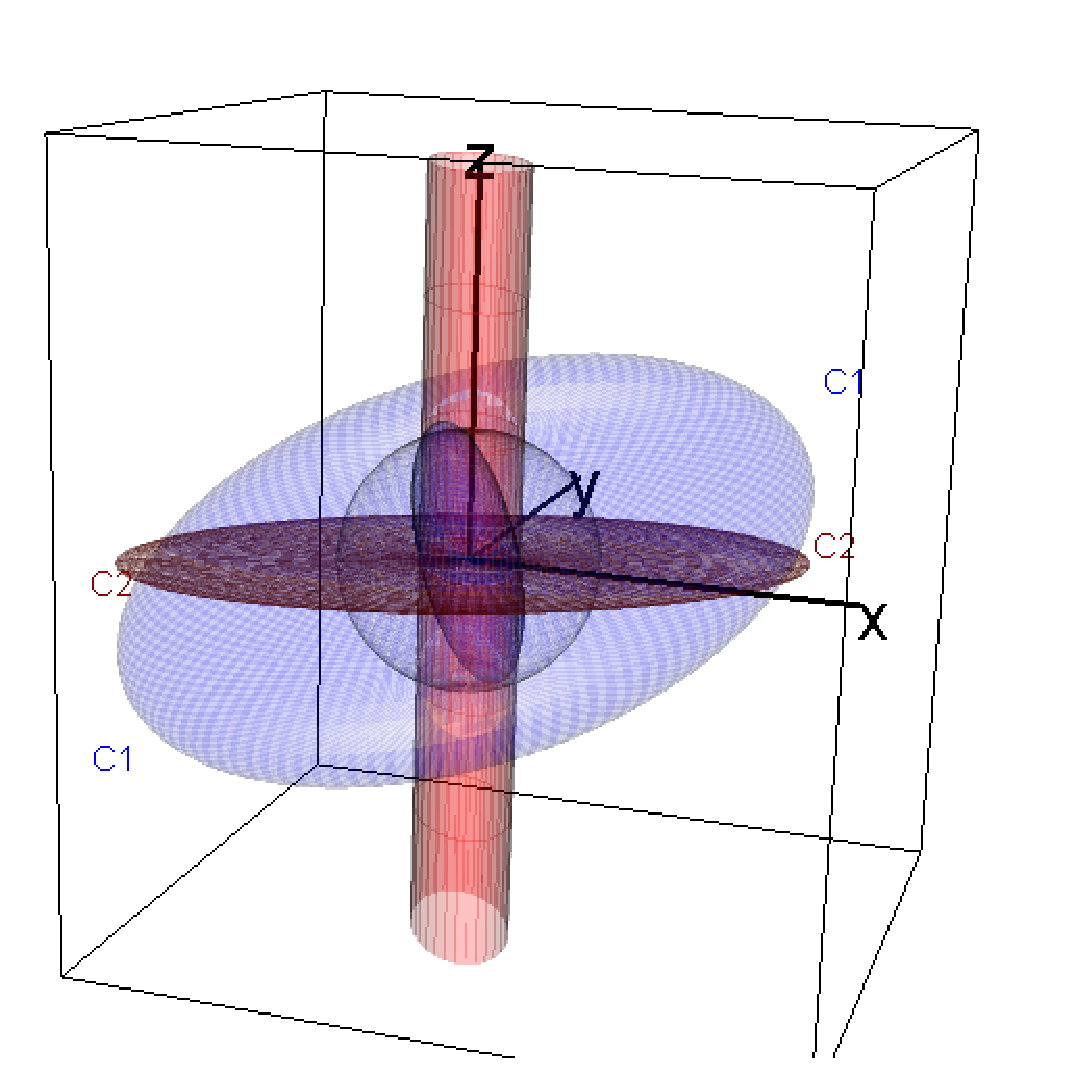
\includegraphics[width=1\linewidth]{fig/gell3d-1}
 \end{minipage}%
 \hfill
 \begin{minipage}[b]{.49\linewidth}
  \centering
  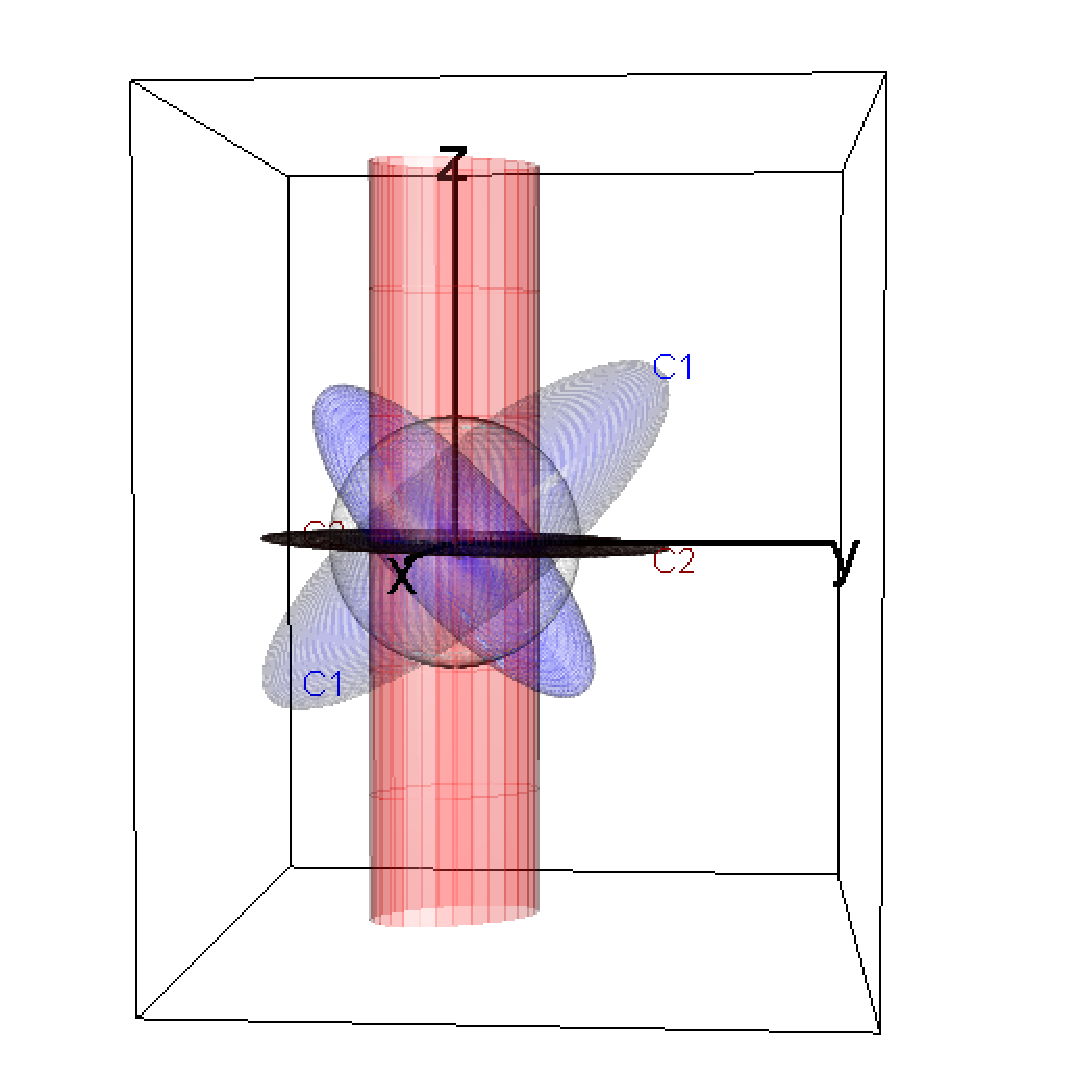
\includegraphics[width=1\linewidth]{fig/gell3d-4}
 \end{minipage}
\caption{Two views of an example of generalized ellipsoids.  $\mat{C}_1$  (blue) determines a proper, fat ellipsoid;
its inverse $\mat{C}_1^{-1}$ also generates a proper ellipsoid. $\mat{C}_2$  (red) determines an improper, flat ellipsoid,
whose inverse $\mat{C}_2^{-1}$ is an unbounded cylinder of elliptical cross section.  The scale of these images is defined
by a unit sphere (gray). The left panel shows that $\mat{C}_2$ is a projection of  $\mat{C}_1$ onto the plane where
$z=0$.
The right panel shows a view illustrating the orthogonality of each $\mat{C}$ and its dual,  $\mat{C}^{-1}$.
}
\label{fig:gell3d}
\end{figure}

The $\mat{U} (\mat{\Delta} \mathcal{S})$ representation also allow us to characterize any such
generalized ellipsoid in $\Real{p}$ by its \emph{signature},
\begin{equation}
 \mathcal{G}(\mat{C}) = \#[ \delta_i >0, \: \delta_i =0, \: \delta_i =\infty ] \quad \mbox{with} \quad \sum \mathcal{G}(\mat{C}) = p\comma
\end{equation}
a 3-vector containing the number ($\#$) of positive, zero and infinite singular values.  For example, in $\Real{3}$, any proper ellipsoid has
the signature $\mathcal{G}(\mat{C})=(3, 0, 0)$; a flat, 2D ellipsoid has $\mathcal{G}(\mat{C})=(2, 1, 0)$; a flat, 1D ellipsoid (a line)
has $\mathcal{G}(\mat{C})=(1, 2, 0)$. Unbounded examples include an infinite flat plane, with $\mathcal{G}(\mat{C})=(0, 1, 2)$,
and an infinite cylinder of elliptical cross-section, with $\mathcal{G}(\mat{C})=(2, 0, 1)$.


\figref{fig:gell3d} illustrates these ideas, using two generating matrices, $\mat{C}_1$ and $\mat{C}_2$, in this more
general representation,
\[
\mat{C}_1 = \left[
\begin{array}{ccc}
 6 & 2 & 1  \\
 2 & 3 & 2  \\
 1 & 2 & 2
\end{array}
\right]
\comma \quad\quad
\mat{C}_2 = \left[
\begin{array}{ccc}
 6 & 2 & 0  \\
 2 & 3 & 0  \\
 0 & 0 & 0
\end{array}
\right]
\]
where $\mat{C}_1$ generates a proper ellipsoid and $\mat{C}_2$ generates an improper, flat ellipsoid.
 $\mat{C}_1$ and its dual,  $\mat{C}_1^{-1}$ both have signatures $(3, 0, 0)$.
$\mat{C}_2$ has the signature $(2, 1, 0)$, while its inverse (dual) has the signature $(2, 0, 1)$.
These varieties of ellipsoids are more easily understood in the 3D movies included in the online supplements.

%\TODO{Check this section: it is complete enough? Could it be trimmed?} 